	\documentclass[journal,12pt,twocolumn]{IEEEtran}\usepackage[margin=1.25 in]{geometry}
\usepackage{amsmath, amssymb}
\usepackage{multicol}
\usepackage{graphicx}
\usepackage[shortlabels]{enumitem}
\usepackage{cases}

\providecommand{\x}[1]{\ensuremath{\text{X}\left(#1\right)}}
\providecommand{\p}[1]{\ensuremath{{P_X}\left(#1\right)}}
\providecommand{\f}[1]{\ensuremath{{F_X}\left(#1\right)}}

\addtolength{\topmargin}{-.4 in}

\title{\LARGE{\textbf{Assignment-4}\\(CBSE 12th Ex 16.3)}}
\author{\normalsize J Sai Sri Hari Vamshi\\ \footnotesize AI21BTECH11014}
\date{}

\begin{document}
\maketitle
\begin{center}
    \textbf{\large example 23:}
\end{center}

\noindent A bag contains $2$ white and $1$ red balls. One ball is drawn at random and then put back into the box after noting its colour. The process is repeated again. If X denotes the number of red balls recorded in the two draws, describe X.

\begin{center}
    \textbf{\large Solution:}
\end{center}

\noindent Let the balls in the bag be denoted by $w_1, w_2$ and $r$ as the two white balls are not identical.
\noindent Then the sample space is:
	\begin{align*}
	S  = \{w_1 w_1,\ w_1 w_2,\ w_2 w_2,\ w_2 w_1,\\ \ w_1 r,\ w_2 r,\ r w_1,\ r 	w_2,\ r r\}
	\end{align*}
\noindent Let $\omega$ be an element of the sample space. i.e.,
	\begin{align*}
	\omega & \in S
	\end{align*}
\noindent Given that X denotes the number of red balls, then 
	\begin{align*}
	\x{\omega} = \text{No. of red balls in }\omega
	\end{align*}
\noindent Therefore,
	\begin{align*}
	\x{\{w_1 w_1\}} = \x{\{w_1 w_2\}} & = 0\\ \x{\{w_2 w_1\}} = \x{\{w_2 w_2\}} & = 0\\
	\x{\{r\ w_1\}} = \x{\{r\ w_2\}} & = 1\\ \x{\{w_1\ r\}} = \x{\{w_2\ r\}} & = 1\\
	\x{\{r\ r\}} & = 2
	\end{align*}
\noindent Thus X is a random variable with values $0,\ 1$ and $2$.\\
\noindent The PMF is given by,
	\begin{align*}
	\p k = 
		\begin{cases}
		\frac{4}{9}, & k = 0\\
		\frac{4}{9}, & k = 1\\
		\frac{1}{9}, & k = 2\\
		\end{cases}		
	\end{align*}
\noindent The CDF can be obtained from PMF by,
	\begin{align*}
	\f k & = \sum_{i = 0}^{i = k}\p i\\
	\end{align*}
\noindent The CDF can be obtaines as,
	\begin{align*}
	\f k = 
		\begin{cases}
			\frac{4}{9}, & k = 0\\
			\frac{8}{9}, & k = 1\\
			1, & k = 2\\			
		\end{cases}
	\end{align*}
\noindent The PMF and CDF Graphs are below,
\begin{center}
		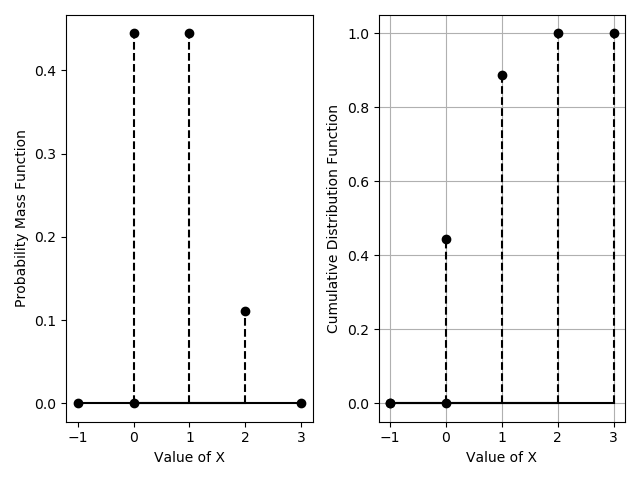
\includegraphics[width = \columnwidth]{figs/f1.png}
	\end{center}
\end{document}